\documentclass[12pt,hyperref,a4paper,UTF8]{ctexart}
\usepackage{HDUReport}
\usepackage{listings}
\usepackage{xcolor}
\usepackage{graphicx}
\usepackage{setspace}
\usepackage{float}
\setstretch{1.5} % 设置全局行距为1.5倍

\usepackage{enumitem} % 载入enumitem包以便自定义列表环境
\setlist[itemize]{itemsep=0pt, parsep=0pt} % 设置itemize环境的项目间距和段落间距

\setmainfont{Times New Roman} % 英文正文为Times New Roman


\usepackage{tikz}
\usetikzlibrary{shapes.geometric, arrows}
\usetikzlibrary{positioning, arrows.meta}
\usetikzlibrary{calc}
%封面页设置
{   
    %标题
    \title{ 
        \vspace{1cm}
        \heiti \Huge \textbf{《单片机原理及应用》作业报告} \par
        \vspace{1cm} 
        \heiti \Large {\underline{实验报告2第三部分:跑马灯闪烁}   } 
        \vspace{3cm}
    
    }

    \author{
        \vspace{0.5cm}
        \kaishu\Large 学院\ \dlmu[9cm]{卓越学院} \\ %学院
        \vspace{0.5cm}
        \kaishu\Large 学号\ \dlmu[9cm]{23040447} \\ %班级
        \vspace{0.5cm}
        \kaishu\Large 姓名\ \dlmu[9cm]{陈文轩} \qquad  \\ %学号
        \vspace{0.5cm}
        \kaishu\Large 专业\ \dlmu[9cm]{智能硬件与系统(电子信息工程)} \qquad \\ %姓名 
    }
        
    \date{\today} % 默认为今天的日期,可以注释掉不显示日期
}
%%------------------------document环境开始------------------------%%
\begin{document}

%%-----------------------封面--------------------%%
\cover
\thispagestyle{empty} % 首页不显示页码
%%------------------摘要-------------%%
%\newpage
%\begin{abstract}




%\end{abstract}

%\thispagestyle{empty} % 首页不显示页码

%%--------------------------目录页------------------------%%
% \newpage
% \tableofcontents
% \thispagestyle{empty} % 目录不显示页码

%%------------------------正文页从这里开始-------------------%
\newpage
\setcounter{page}{1} % 让页码从正文开始编号

%%可选择这里也放一个标题
%\begin{center}
%    \title{ \Huge \textbf{{标题}}}
%\end{center}

\section{原题目}

\textbf{通过软硬件设计实现8个LED灯单灯其他形式跑马灯(选做)。用Proteus软件仿真。用C语言编程。}

\section{实验程序}
\begin{lstlisting}[language=C, caption={跑马灯实验程序}]
#include <reg51.h>
#include <intrins.h> // 包含_crol_函数

#define LED_PORT P1
#define DELAY_MS 150 // 控制跑马灯速度

void delay(unsigned int ms) {
    unsigned int i, j;
    for(i=0; i<ms; i++)
        for(j=0; j<114; j++); //阻塞式延时一段时间
}

void main() {
    unsigned char led_pattern = 0x01; // 初始模式:0000_0001(第一个LED亮)
    
    while(1) {
        LED_PORT = led_pattern;
        delay(DELAY_MS); //软件阻塞式延时
        
        // 左移跑马灯(低电平有效)
        led_pattern = _crol_(led_pattern, 1);
        
    }
}  
\end{lstlisting}

\section{实验效果}

\begin{figure}[H] % [H] 表示强制当前位置插入
    \centering
    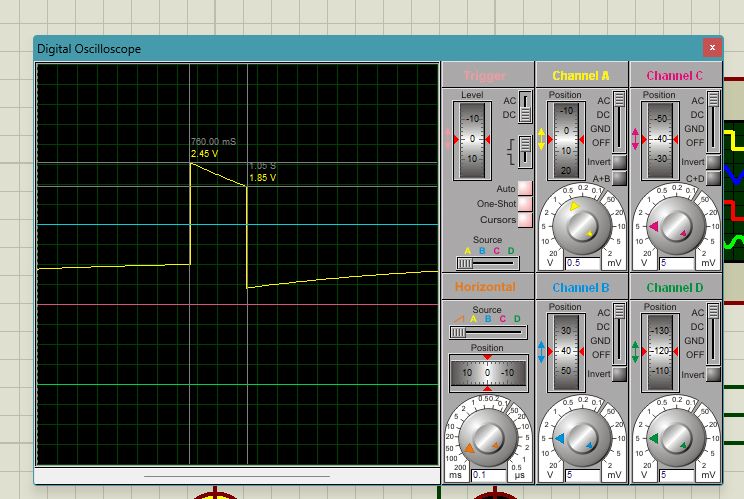
\includegraphics[width=0.8\textwidth]{figures/201.png} % 调整宽度为文本宽度的 80%
    \caption{Proteus示波器跑马灯效果,脉宽手动测量约290mS} % 图片标题
    \label{fig:example} % 图片标签,用于引用
\end{figure}

\begin{figure}[H] % [H] 表示强制当前位置插入
    \centering
    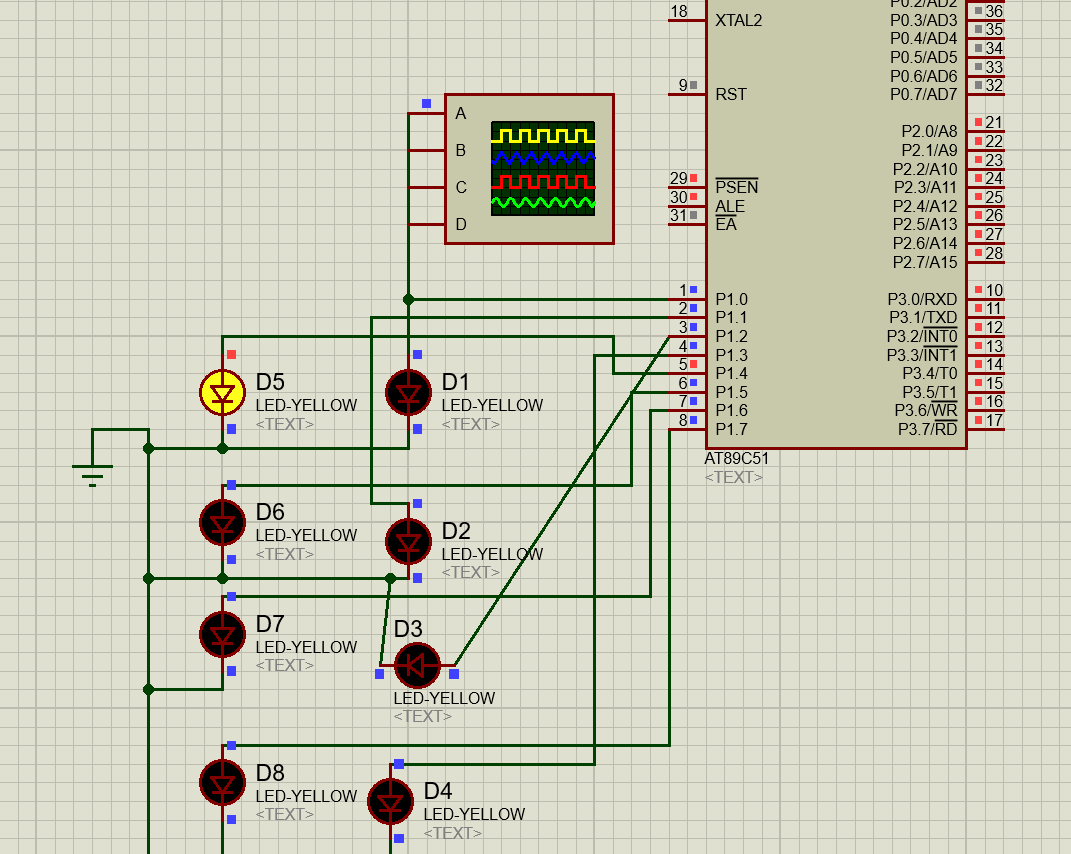
\includegraphics[width=0.8\textwidth]{figures/202.png} % 调整宽度为文本宽度的 80%
    \caption{Proteus灯1灭效果} % 图片标题
    \label{fig:example} % 图片标签,用于引用
\end{figure}

\begin{figure}[H] % [H] 表示强制当前位置插入
    \centering
    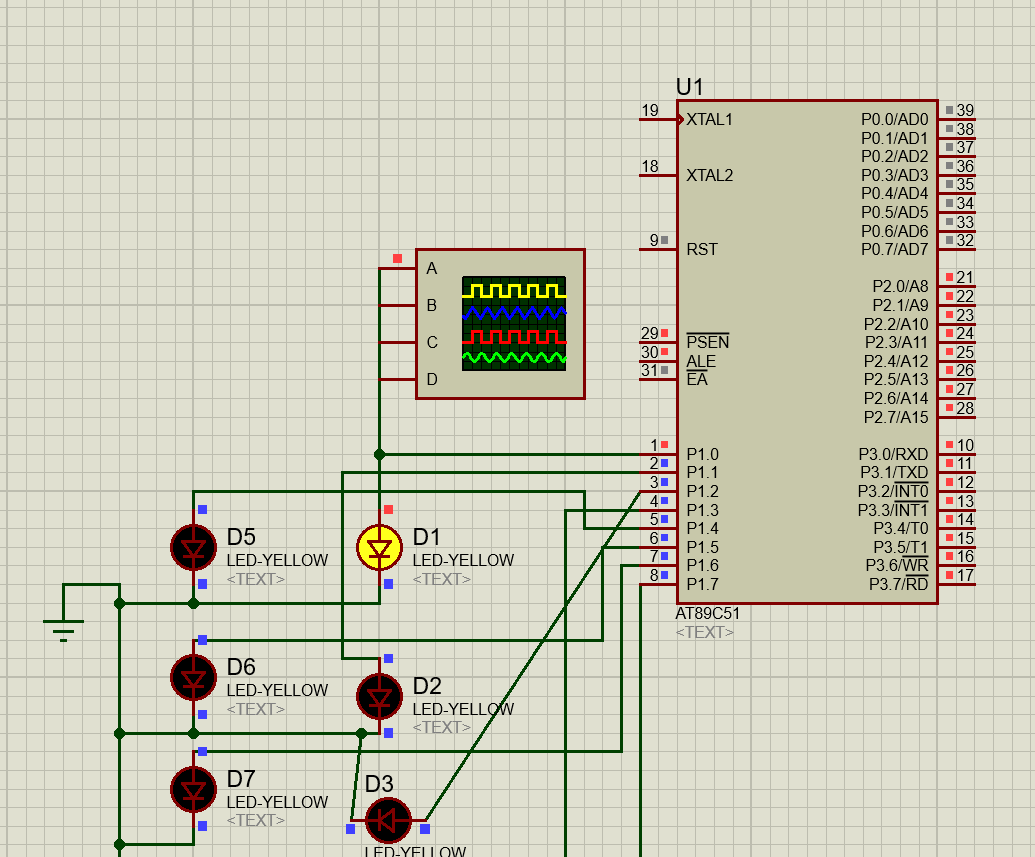
\includegraphics[width=0.8\textwidth]{figures/203.png} % 调整宽度为文本宽度的 80%
    \caption{Proteus灯1亮效果} % 图片标题
    \label{fig:example} % 图片标签,用于引用
\end{figure}



\section{流程图}

\begin{figure}[H]
    \centering
    \begin{tikzpicture}[
        node distance=1.5cm,
        startstop/.style={rectangle, rounded corners, minimum width=3cm, minimum height=1cm, text centered, draw=black, fill=red!30},
        process/.style={rectangle, minimum width=3cm, minimum height=1cm, text centered, draw=black, fill=blue!30},
        decision/.style={diamond, aspect=1.8, minimum width=2.5cm, minimum height=1.8cm, text centered, draw=black, fill=green!30},
        arrow/.style={thick, -Stealth}
    ]

        % ===== 主流程 =====
        \node (start) [startstop] {程序开始};
        \node (initLED) [process, below=of start] {初始化 LED 模式};
        \node (mainLoop) [process, below=of initLED] {主循环};
        \node (updateLED) [process, right=3cm of mainLoop] {更新 LED 状态};
        \node (delay) [process, below=of updateLED] {延时 150ms};
        \node (repeat) [decision, right=3cm of delay] {继续循环?};

        % ===== 箭头连接 =====
        \draw [arrow] (start) -- (initLED);
        \draw [arrow] (initLED) -- (mainLoop);
        \draw [arrow] (mainLoop) -- (updateLED);
        \draw [arrow] (updateLED) -- (delay);
        \draw [arrow] (delay) -- (repeat);
        \draw [arrow] (repeat.north) -- ++(0,2.5cm) -| (mainLoop.east) node[pos=0.25, right] {是};
        \draw [arrow] (repeat.south) -- ++(0,-1cm) node[right] {否};

    \end{tikzpicture}
    \caption{跑马灯程序流程图}
    \label{fig:led_flowchart}
\end{figure}



\section{实验体会}

通过本次实验,我对 51单片机 的基本功能和应用有了更深入的理解,初步使用了crol函数,实现了定时阻塞式控制,从而控制了 LED 的亮灭脉宽。




\end{document}